\documentclass[10pt]{article}
\usepackage[frenchb,english]{babel}
\usepackage{multirow}
\usepackage{graphicx}
\usepackage{calc}
\usepackage{caption}
\usepackage{array}
\usepackage{booktabs}
\usepackage{amsmath}
\usepackage{rotating}
\usepackage{tikz}
\usepackage{tabularx}
\usepackage{booktabs}
\usetikzlibrary{positioning,calc}
\newcommand{\defineWidthHeight}[2]{

\newcounter{margin}
\newcounter{Paperwidth}
\newcounter{Paperheight}

\setcounter{margin}{2}
\setcounter{Paperwidth}{#1}
\setcounter{Paperheight}{#2} 

\usepackage[margin=\themargin mm]{geometry}
\setlength{\paperwidth}{\thePaperwidth mm} 
\newcounter{Textwidth}
\setcounter{Textwidth}{\value{Paperwidth}-2*\value{margin}}
\setlength{\textwidth}{\value{Textwidth} mm}
\setlength{\paperheight}{\thePaperheight mm} 
\newcounter{Textheight}
\setcounter{Textheight}{\value{Paperheight}-2*\value{margin}}
\setlength{\textheight}{\value{Textheight} mm}
\setlength{\parindent}{0mm}
}
\fontfamily{phv}\selectfont
\setlength{\parindent}{0cm}
%%%%%%%%%%%%%%%%%%%%%%%%%%%%%%%%%%%%%%%%%%%%%%%%%%%%%%%%%%%%%%%%%%%%%%%%%
% Command to automatically crop the pdf file
%%%%%%%%%%%%%%%%%%%%%%%%%%%%%%%%%%%%%%%%%%%%%%%%%%%%%%%%%%%%%%%%%%%%%%%%%
\newcommand\cropped[2]{%
    \immediate\write18{pdfcrop #1.pdf #1_cropped.pdf}%
    \includegraphics[width=#2\textwidth]{#1_cropped.pdf}}
%%%%%%%%%%%%%%%%%%%%%%%%%%%%%%%%%%%%%%%%%%%%%%%%%%%%%%%%%%%%%%%%%%%%%%%%%
\defineWidthHeight{190}{210}
\usepackage[percent]{overpic}

\begin{document}
\fontfamily{phv}\selectfont
\def\raiseS[#1]{\raisebox{2\height}{#1}}
\def\coll{0.31\textwidth}
\def\up{3.5}
%-----------------------------------------------------------------------------------------------------------------------------------------------------------------------
% Set path of  code here (i.e. where plots are exported)
%-----------------------------------------------------------------------------------------------------------------------------------------------------------------------
\graphicspath{
{../../code/mechanistic/PFS_thresholds/}
{../../code/statistical_analysis/PFS/}
}	
%-----------------------------------------------------------------------------------------------------------------------------------------------------------------------
%\raisebox{4.8cm}{\textbf{A}}
\begin{tabular}{ccc}
\textbf{Gender}
&
\textbf{MYCN status}
&
\textbf{Age}
\\[1ex]
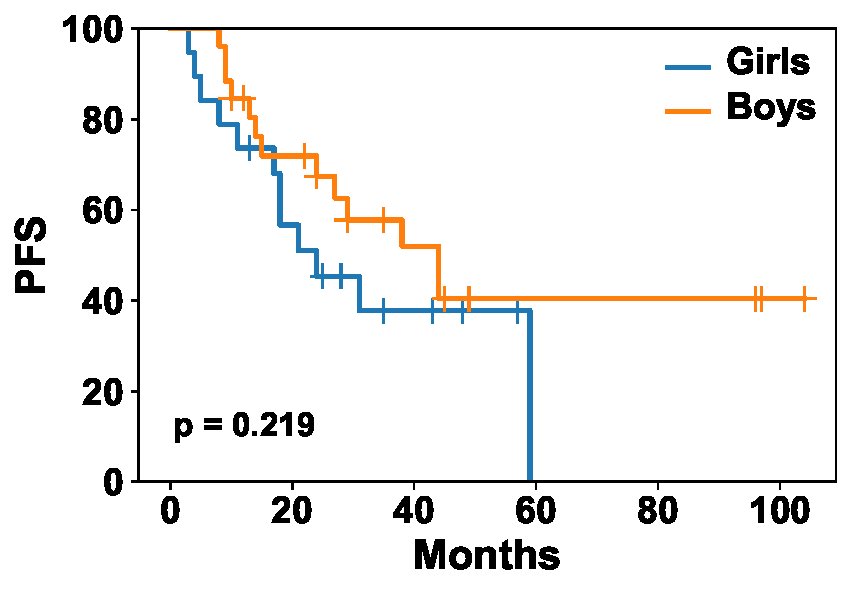
\includegraphics[width=\coll]{sex}
&
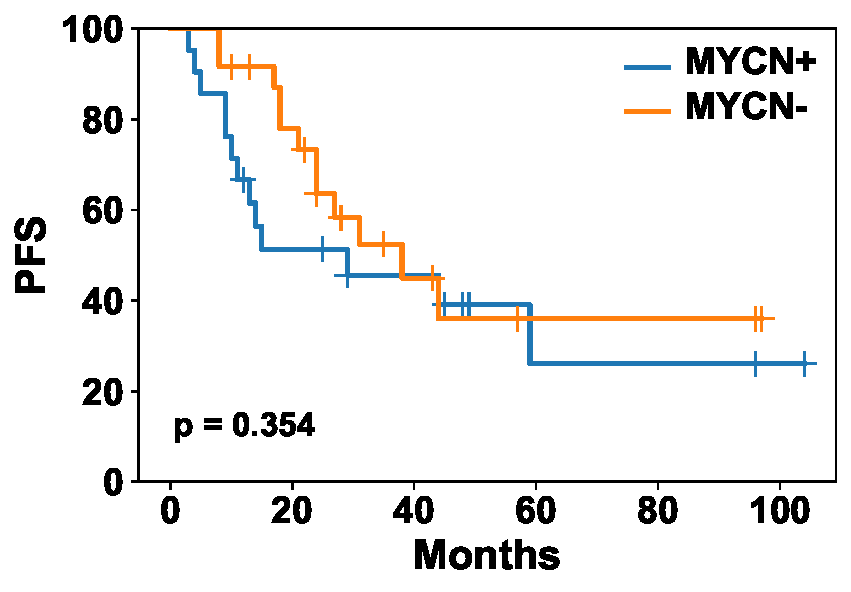
\includegraphics[width=\coll]{Nmyc}
&
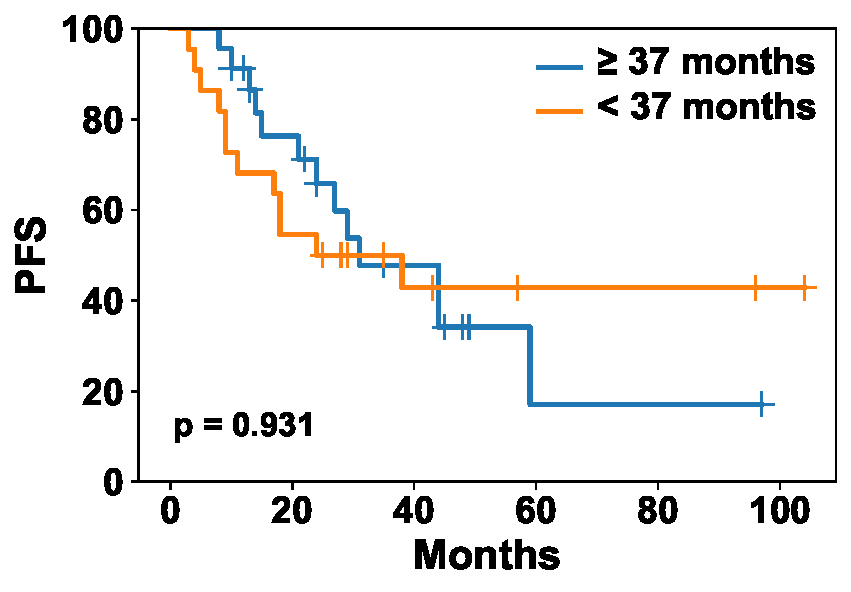
\includegraphics[width=\coll]{age_percentiles/50}
\\[2ex]
\textbf{LDH median}
&
\textbf{LDH literature cut-off}
&
\textbf{LDH 80$^{th}$ percentile}
\\[1ex]
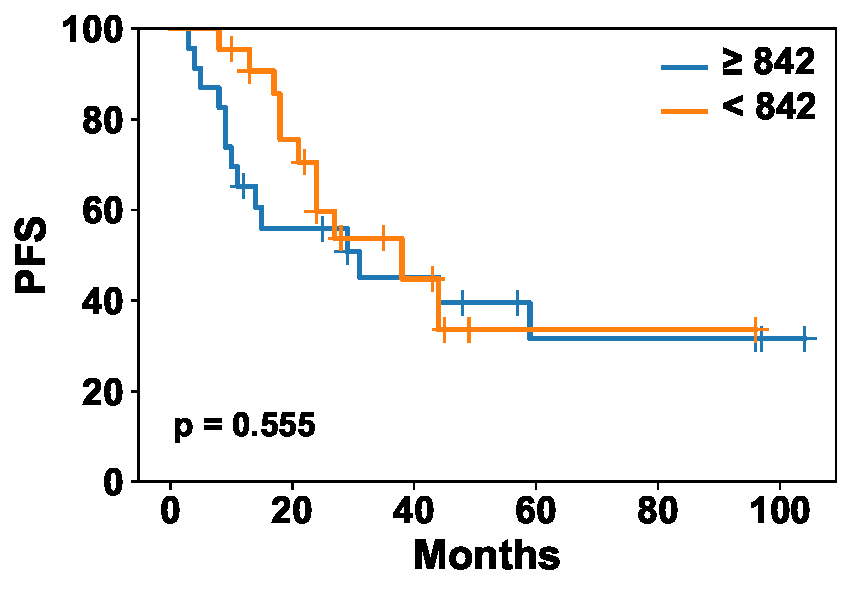
\includegraphics[width=\coll]{LDH_percentiles/50}
&
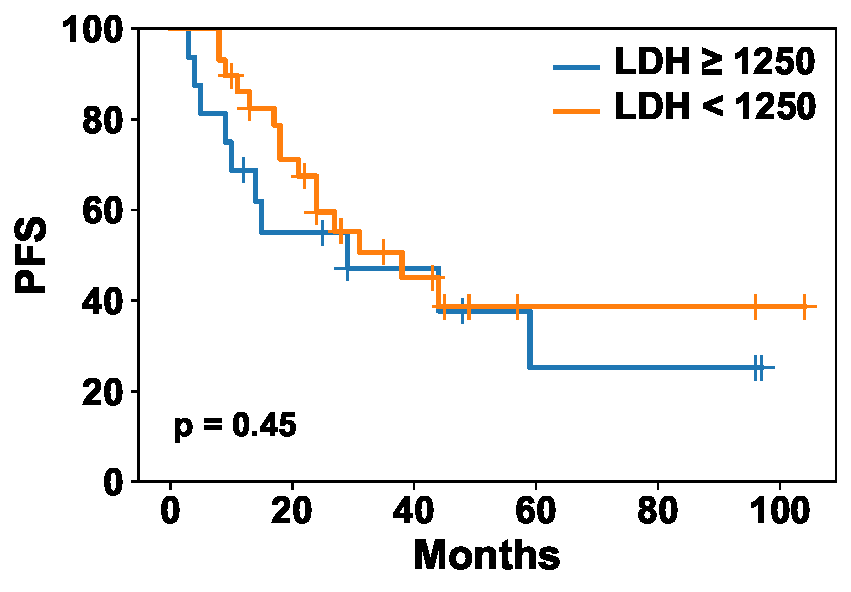
\includegraphics[width=\coll]{LDH}
&
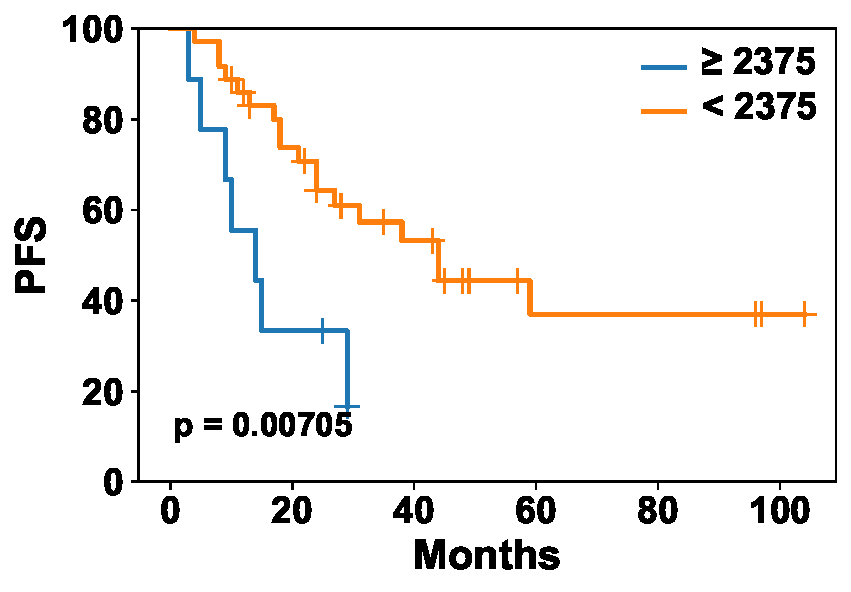
\includegraphics[width=\coll]{LDH_percentiles/80}
\\[2ex]
\textbf{SIOPEN median}
&
\textbf{SIOPEN literature cut-off}
&
\textbf{SIOPEN 90$^{th}$ percentile}
\\[1ex]
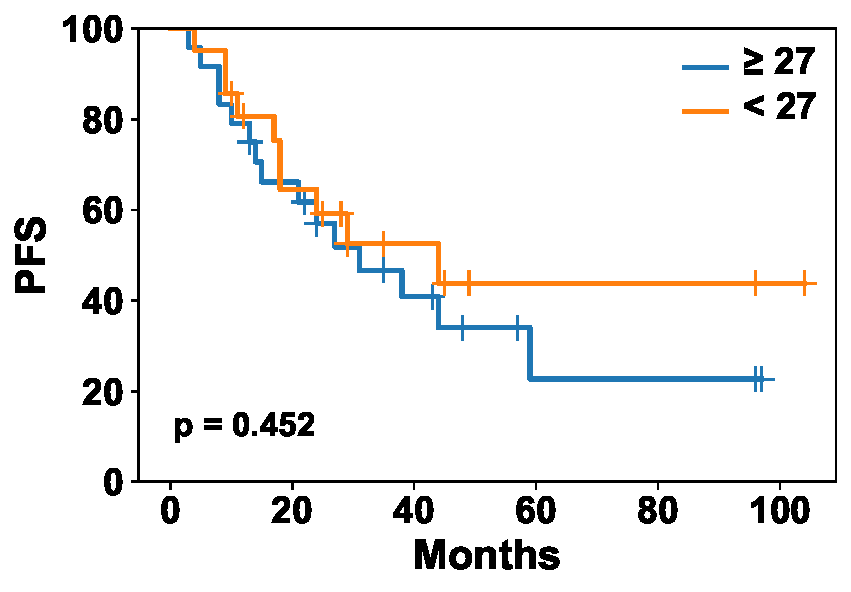
\includegraphics[width=\coll]{SIOPEN_percentiles/50}
&
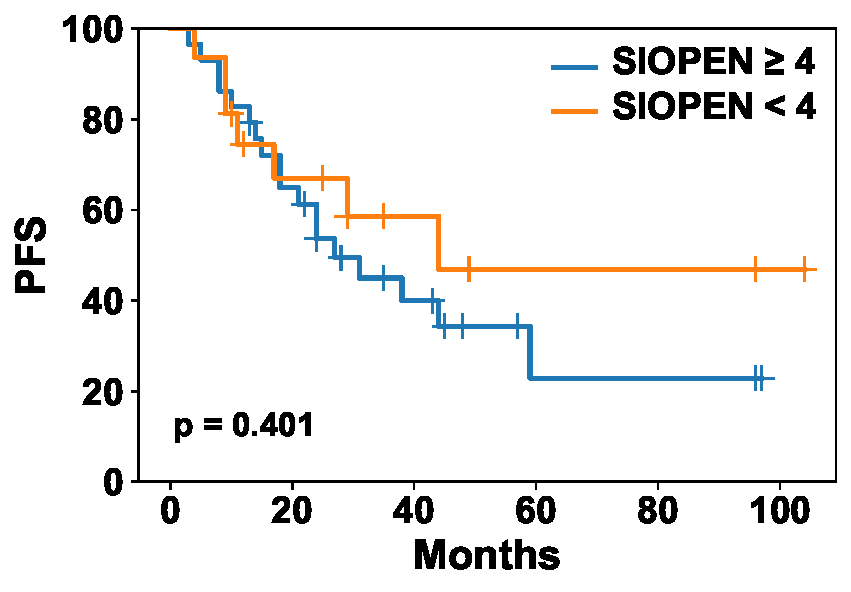
\includegraphics[width=\coll]{SIOPEN}
&
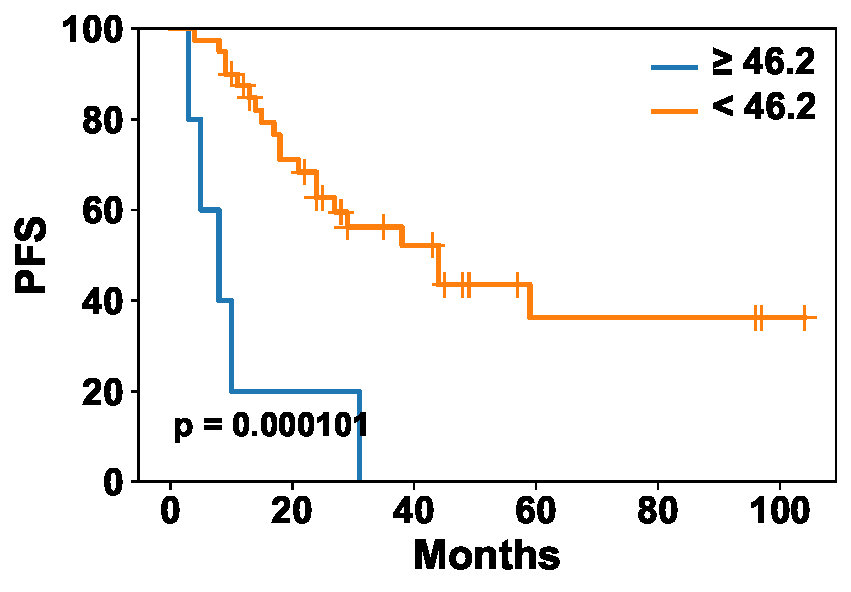
\includegraphics[width=\coll]{SIOPEN_percentiles/90}
\\[2ex]
\textbf{Tumor size median}
&
\textbf{$\mu$ median}
&
\textbf{$S_{vis}$ median}
\\[1ex]
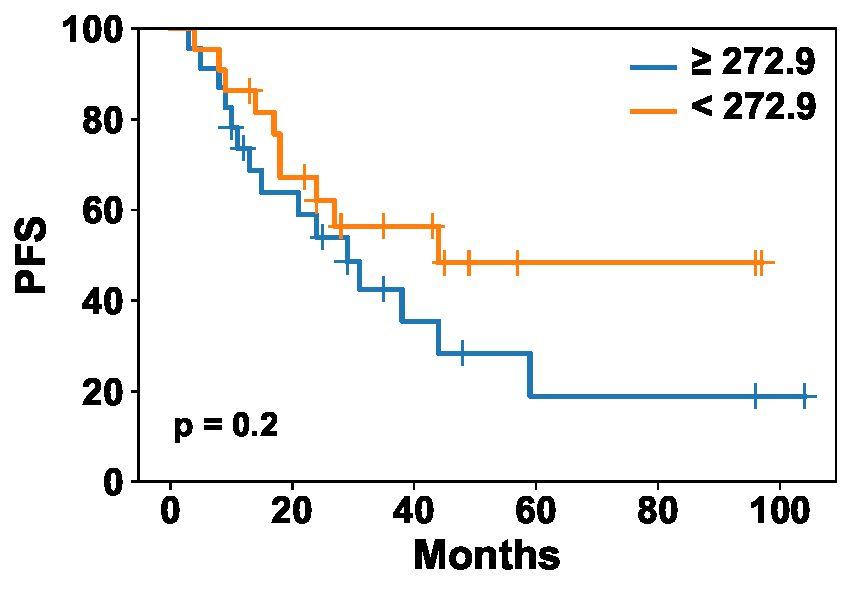
\includegraphics[width=\coll]{tumor_size_percentiles/50}
&
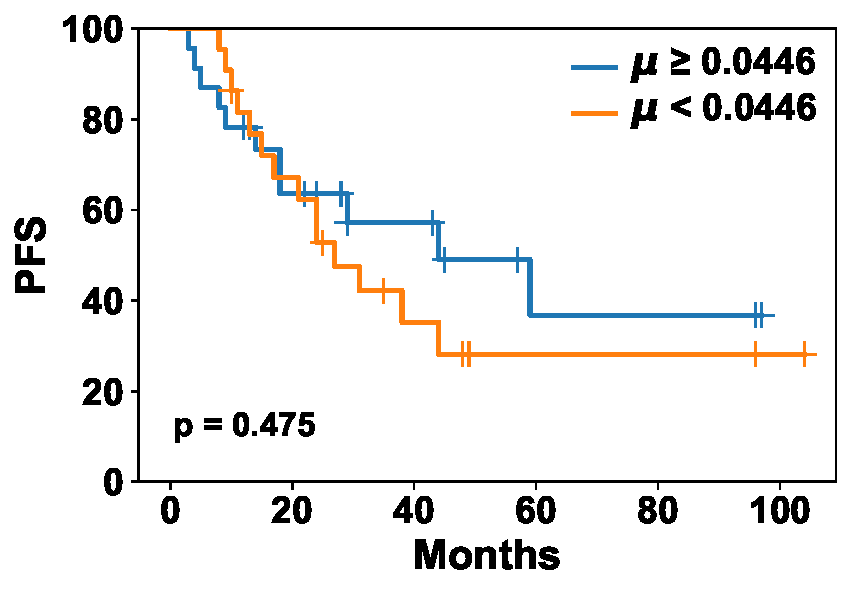
\includegraphics[width=\coll]{mu/median}
&
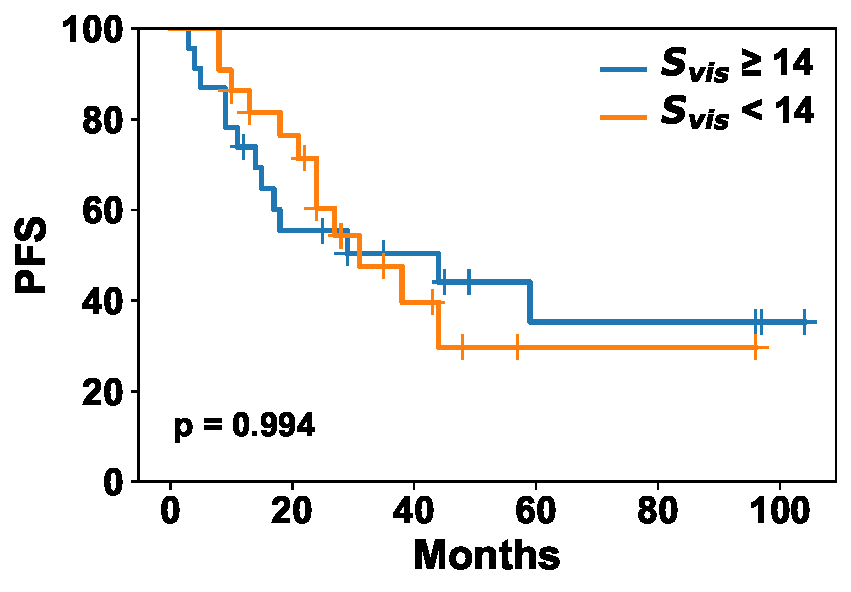
\includegraphics[width=\coll]{visible_threshold/median}
\end{tabular}
\end{document}